
\documentclass[12pt]{report}
\usepackage[utf8]{inputenc}

\usepackage{geometry}
\usepackage[spanish]{babel}
\renewcommand{\baselinestretch}{1.5}
\geometry{letterpaper, margin=2.5cm}
\usepackage{graphicx}
\usepackage{hyperref}
\urlstyle{same}
\usepackage{fancyhdr}
\usepackage{amsmath}
\usepackage{braket,mleftright}
\mleftright
 
\usepackage[sorting=none]{biblatex}
 
\addbibresource{references.bib}

\begin{document}

\begin{titlepage}
   \begin{center}
       \vspace*{1cm}
       
       
       \large
       \textbf{Estimación de la contribución del \textit{forward scattering} de muones en la señal registrada por el detector MuTe}
       
       %\large
       %\vspace{0.5cm}
        %¿Subtítulo?
 
       \vspace{1.5cm}
 
       \small
       Propuesta de tesis de pregrado para optar al título de \\
       Físico
       
       
       \normalsize
       \textbf{Ricardo de León Barrios}
       
       \small
       \vspace{1cm}
       Director\\
       \textbf{Mauricio Suárez Durán}$^{1,2}$\\
       Doctor en Ciencias Naturales (Física)
       
       \vspace{1cm}
       Codirector\\
       \textbf{Luis A. Núñez de Villavicencio}$^1$\\
       Doctor en Física\\
       
       \vspace{1cm}
       $^1$\textit{Grupo de Investigación en Relatividad y Gravitación, UIS}\\
       $^2$\textit{Grupo de Investigación Integrar, Universidad de Pamplona}
 
       \vfill
       
       
 
       %\vspace{0.8cm}
 
       
 
       \small
       Escuela de Física\\
       Facultad de Ciencias\\
       Universidad Industrial de Santander\\
       Bucaramanga, Colombia\\
       2020\\
       \vspace{0.3cm}
       
\includegraphics[width=0.25\textwidth]{logo/logoUIS.png}
 
   \end{center}
\end{titlepage}

%---------------------------------------

\section*{Resumen}

La muografía es una técnica por la cual se obtienen imágenes de un volumen mediante la detección de variaciones en el flujo de muones que lo atraviesan. Uno de sus principales usos en los últimos años ha sido el de conseguir imágenes del interior de estructuras geológicas, principalmente volcanes, usando detectores Cherenkov. En esta aplicación, uno de los fenómenos que afecta la obtención de imágenes es el \textit{forward scattering} (lit. ``dispersión hacia adelante''), en el que muones incidentes sobre la superficie de la estructura estudiada interactúan con ella y se ven deflectados. Estos muones dispersados pueden llegar al detector y corromper la señal deseada de los muones de fondo. Este trabajo apunta a estimar el efecto del \textit{forward scattering} de muones sobre el detector MuTe, un observatorio híbrido que combina un hodoscopio con un detector Cherenkov de agua, con el fin de caracterizar el ruido que este pueda representar sobre la señal en el detector. Se hará uso de las herramientas computacionales CORSIKA y MAGNETOCOSMICS para simular el flujo de muones atmosféricos a nivel del suelo, y Geant4 para simular la interacción de estos muones con la superficie, el fenómeno del \textit{forward scattering} y su efecto en la señal de un detector.


%------------------------------------
\section*{Introducción}



La muografía ha despertado el interés de la comunidad científica en los últimos años debido a su gran poder en aplicaciones de escaneo de grandes estructuras.

El principio en el que se basa la muografía es sencillo: similar a como los rayos x en medicina se atenúan en distintos valores cuando pasan por las diferentes estructuras internas del cuerpo, el flujo de muones sobre un detector también varía en función de la cantidad de materia que los muones han atravesado en su trayectoria. El uso de muones presenta una importante ventaja para el escaneo de estructuras geológicas debido al gran poder penetrativo de estas partículas así como al hecho de que están fácilmente disponibles en grandes cantidades: los muones están siendo creados constantemente en la atmósfera terrestre debido a la interacción de rayos cósmicos con partículas de aire, en procesos llamados \textit{cascadas atmosféricas extensas}.

Por su parte, el \textit{forward scattering} de muones es un fenómeno en el que estas partículas cambian su dirección al interactuar con una superficie sólida. Al ser deflectados, es posible que estos muones terminen siendo registrados en un detector durante una toma de datos de muografía.

En este proyecto se estimará el efecto que el fenómeno de \textit{forward scattering} de muones atmosféricos tiene sobre la señal de un detector para muografía (específicamente el MuTe), el cual se ha descrito como una potencial fuente de ruido irreducible \cite{gomez2017forward}. Este documento de propuesta de tesis se divide en las siguientes secciones: Una sección de \textbf{Planteamiento del problema y justificación}, donde se explicará el problema que se pretende atacar y el propósito con el que se hace; un \textbf{Marco teórico}, donde se exponen algunos conceptos básicos de la teoría concerniente a la problemática que se desea abordar; la sección de \textbf{Objetivos}, donde se exponen los objetivos del trabajo de grado que se desean alcanzar, y la sección de \textbf{Metodología}, donde se enumeran las actividades a seguir para el desarrollo ordenado del trabajo junto con el debido cronograma.


%-------------------------------------------
\section*{Justificación y planteamiento del problema}

La muografía de volcanes es una técnica para estimar la distribución de densidad de materia al interior de un edificio volcánico. Esto se logra a partir del análisis del registro del flujo de muones que atraviesan la estructura; en particular, determinando las diferencias de flujo en función de la dirección o posición en el volcán por la que han atravesado. En este contexto, es fundamental para la correcta interpretación de los datos determinar qué mediciones no están correlacionadas con la estructura, o no provienen de esta.

En el escenario de la muografía, es común el uso de detectores Cherenkov y hodoscopios. Con detectores Cherenkov se puede detectar el paso de partículas energéticas, como los muones, basándose en el fenómeno de emisión de radiación Cherenkov, mientras que con hodoscopios se puede hacer una recreación de la trayectoria de las partículas incidentes. Con esto en mente, la Universidad Industrial de Santander y colaboradores han estado trabajando en el proyecto MuTe\footnote{\textit{\textbf{Mu}on \textbf{Te}lescope}}: la implementación de un detector de muones híbrido que combine los principios de funcionamiento de un hodoscopio con un detector Cherenkov de agua (WCD\footnote{\textit{Water Cherenkov Detector}}) para el escaneo de estructuras geológicas en las montañas de Colombia \cite{pena2019calibration}\cite{rodriguez2018minimute}. En representación de Colombia, la UIS realiza el estudio del clima espacial y la coordinación de proyectos de implementación de detectores como el MuTe para mediciones de radiación cósmica a nivel del suelo dentro del marco del proyecto LAGO\footnote{\textit{Latin American Giant Observatory}, \url{http://lagoproject.net/}}. Supervisado por la Colaboración LAGO, una colaboración entre más de 100 científicos en 30 instituciones de 11 países distintos (en su mayoría latinoamericanos\footnote{Los países que participan en la Colaboración LAGO son Argentina, Bolivia, Brasil, Chile, Colombia, Ecuador, Guatemala, México, Perú y Venezuela en Latinoamérica, y España en Europa.}), el proyecto LAGO pretende servir como un gran observatorio de astropartículas, haciendo investigación en temas de Universo extremo, clima espacial y radiación atmosférica a nivel del suelo. En particular, uno de los objetivos del proyecto MuTe es estudiar la estructura de los volcanes activos en Colombia. Estudiando las distribuciones de densidad en los volcanes activos del país, se espera obtener modelos de sus estructuras internas que, potencialmente, permitan evaluar los riesgos futuros que estos puedan representar. Para esto, se busca que las imágenes obtenidas de los volcanes por tomografía de muones sean lo más detalladas posibles, siendo entonces importante reducir tanto como sea posible los efectos del ruido en los detectores. Hasta la fecha, se ha considerado al Cerro Machín, un pico volcánico ubicado en Tolima, como el único apto para la muografía volcánica en Colombia \cite{vesga2018inversion}\cite{balaguera2017astroparticle}.


Cuando se hace muografía de estructuras geológicas, existen varias fuentes de señal que pueden afectar la imagen: hadrones cargados y electrones y positrones, conocidos como \textit{muones falsos} (\textit{fake muons}), y los llamados \textit{muones suaves} (\textit{soft muons}) que se ``reflejan'' en la superficie escaneada y llegan al detector, como se muestra en la figura \ref{fig:scatteredNoise}. También pueden llegar muones por detrás del detector (\textit{backward muons}), quienes igualmente podrían sumar al ruido de fondo \cite{bonechi2020atmospheric}. El MuTe puede discrimar electrones/positrones de muones mediante técnicas de identificación de partículas. Por ejemplo, como se ve en simulaciones hechas en (A Vesga Ramírez y col. 2017) \cite{asorey2017muon}, la gran mayoría de positrones y electrones se encuentran en un rango energético inferior a los muones. Aplicando un umbral a la energía de las partículas recolectadas por el detector se puede reducir en gran medida el efecto de los electrones y positrones en la imagen. Reducir el efecto del ruido generado por los muones dispersados por \textit{forward scattering} es un poco más complejo. En general, el efecto de los muones dispersados es insignificante a altas energías pero cobra importancia a bajas energías. Estos muones dispersados de bajas energías llegan al detector donde se reconstruye su trayectoria, la cual apunta de vuelta a la estructura estudiada, haciendo que se mimeticen con aquellos muones que sí atravesaron el objeto, alterando nuestra percepción de su densidad en esa dirección. Debido a que estas partículas son también muones, no pueden ser descartados del conteo detectado mediante técnicas de identificación de partículas, representando potencialmente un ruido irreducible \cite{gomez2017forward}.

\begin{figure}
    \centering
    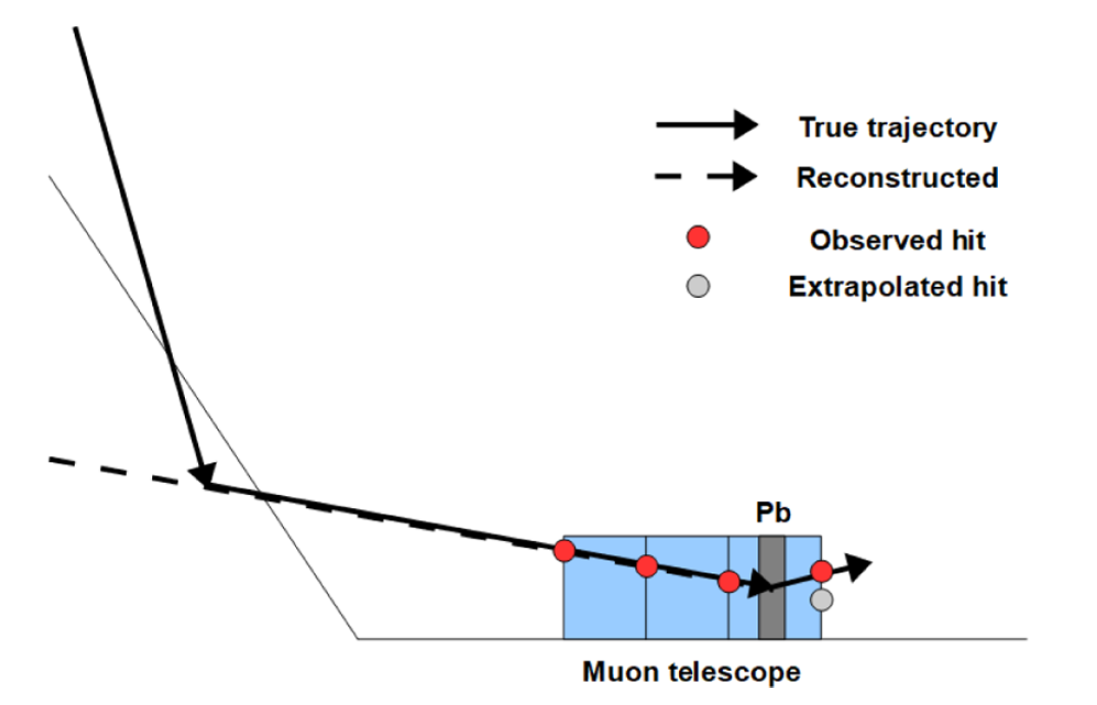
\includegraphics[width=3.5in]{images/scatteredNoiseV2.png}
    \caption{Muon dispersado por la superficie del volcán genera ruido en el WCD. Imagen tomada de (L Bonech y col. 2020) \cite{bonechi2020atmospheric}.}
    \label{fig:scatteredNoise}
\end{figure}


En este trabajo abordaremos el problema asumiento que el detector MuTe registra dos señales principales: una señal de fondo producida por las partícuas secundarias de rayos cósmicos y una señal producida por el \textit{forward scattering} de muones. En el proyecto, apuntaremos a estimar qué tan significativa es la contribución de esta última a la señal de fondo registrada por el MuTe, específicamente aplicado para la muografía volcánica en el Cerro Machín. En (H Gómez y col. 2017)  \cite{gomez2017forward} se discuten algunos efectos del \textit{forward scattering} de muones sobre un detector Cherenkov, donde este fenómeno fue simulado mediante Geant4; sin embargo, el flujo incidente de muones fue generado artificialmente teniendo control total sobre sus valores iniciales de energía y ángulo de incidencia. En cambio, en este proyecto caracterizaremos los efectos del \textit{forward scattering} para muones producidos por rayos cósmicos en la atmósfera, para lo cual será necesaria la implementación de otras herramientas computacionales como CORSIKA y MAGNETOCOSMICS para simular los eventos de cascadas atmosféricas extensas. Con esto, se busca ayudar a que los mapas de densidad de estructuras volcánicas registrados por el MuTe sean lo más prolijos posible, facilitando su estudio y permitiendo, potencialmente, una valoración detallada de los posibles riesgos que estos puedan suponer para la población.





%--------------------------
\section*{Marco teórico}

\subsection*{Sobre rayos cósmicos y cascadas atmosféricas extensas}

\normalsize

Los rayos cósmicos son partículas  altamente energéticas provenientes del espacio. Se pueden clasificar entre aquellas provenientes de nuestro propio Sol y de fuentes externas al sistema solar, ya sea dentro de la Vía Láctea, o de fuentes extragalácticas \cite{moldwin2008introduction}. A pesar de que se les denomina \textit{rayos}, comúnmente se excluye de esta definición a la radiación electromagnética \cite{NASACosmicopia}, limitándose exclusivamente a partículas con masa. La mayoría de los rayos cósmicos están compuestos por núcleos de elementos que van desde el más ligero, el hidrógeno, hasta núcleos de elementos pesados, como el hierro. También se incluyen otras partículas como electrones, neutrones, neutrinos, positrones y antiprotones \cite{NASAImagine}.

Las partículas de rayos cósmicos pueden llegar a alcanzar energías muy altas, de entre 100 MeV y 10 GeV, y velocidades hasta de más del 99\% de la velocidad de la luz \cite{moldwin2008introduction}. Estas partículas, formadas en eventos astrofísicos como llamaradas solares y supernovas, se denominan \textbf{partículas primarias}. Cuando llegan a la atmósfera terrestre interactúan con moléculas de aire (principalmente nitrógeno, oxígeno y argón, que son los mayores componentes de la atmósfera) y decaen en \textbf{partículas secundarias}, creando eventos llamados \textit{cascadas atmosféricas extensas}, o \textit{EAS}\footnote{\textit{Extensive Air Showers}.}. Estas partículas secundarias tienen menos energía que las primarias que las crearon. Algunas partículas secundarias que se pueden formar en estas cascadas son piones y kaones, que a su vez, pueden decaer en muones y neutrinos \cite{grieder2010extensive}. También se pueden formar cascadas electromagnéticas (fotones), partículas alfa, protones, electrones y neutrones.

Para el estudio de los rayos cósmicos es importante la noción de flujo, que se define como el número de partículas que atraviesan una superficie por unidad de área, por unidad de tiempo. En el caso del flujo de rayos cósmicos en la parte superior de la atmósfera, existen varios factores que lo pueden afectar, tales como la actividad solar y el campo magnético terrestre \cite{PhysRevD.98.030001}.

De particular interés en la actualidad es el estudio del flujo de muones, con importantes aplicaciones para escaneos por radiografía y tomografía. Los muones generalmente se forman por el decaimiento de piones, quienes a su vez se crean a partir del choque de núcleos atómicos de rayos cósmicos con partículas de la atmósfera. Los muones son bastante inestables, decayendo rápidamente por interacción débil. El tiempo de vida de los muones, medido en un marco de referencia inercial en reposo respecto a ellos, solo permitiría una distancia de viaje de menos de 500 metros para la mitad de estos (viajando al 99,97\% de la velocidad de la luz) antes de decaer en otras partículas; esto es sin tener en cuenta los efectos relativistas. Sin embargo, debido a las altas velocidades que alcanzan los muones, se deben tener en cuenta los efectos de la contracción de longitudes y la dilatación del tiempo. En este caso, desde nuestra perspectiva en la Tierra, la semivida de los muones se extiende debido a la dilatación temporal, siendo lo suficientemente larga como para detectarlos en la superficie de la Tierra, e incluso a varios cientos de metros bajo tierra, debido a su alto poder penetrativo. Desde la perspectiva de un marco de referencia inercial en reposo respecto de los muones, actúa la contracción espacial, haciendo que la distancia de viaje hacia la superficie de la Tierra sea más corta \cite{cunningham2019high}.

Dos principales métodos de detección de rayos cósmicos existen: uno de detección directa de las partículas primarias en la parte superior de la atmósfera, mediante el uso de globos de grandes altitudes y satélites, y un segundo método, que consiste en detectar, a nivel del suelo, las partículas secundarias y la radiación electromagnética creadas en las EAS. Estas formas de detección son denominadas detección \textit{directa} e \textit{indirecta}, respectivamente. El presente trabajo de investigación se asienta sobre el método de detección indirecta a nivel del suelo.

Una de las herramientas más importantes en la detección de partículas secundarias es el detector Cherenkov, cuyo funcionamiento se basa en el fenómeno de la radiación de Cherenkov: Así llamada por el físico soviético Pável Cherenkov, es la radiación electromagnética emitida cuando un medio dieléctrico es atravesado por una partícula cargada viajando a una velocidad superior a la de la luz en ese medio \cite{jelley1955cerenkov}. Este fenómeno se puede entender como un análogo electromagnético a la onda de choque que se crea cuando un objeto viaja a una velocidad que supera a la velocidad del sonido en un medio.

%---------------------------------------------------------


\subsection*{Sobre la muografía}

La muografía (lit. 'escribir con muones') es el uso de muones cósmicos de altas energías para aplicaciones de escaneo. La muografía ha despertado el interés de la comunidad científica, realizándose importantes avances en esta tecnología en las últimas dos décadas y desarrollando aplicaciones tanto comerciales como académicas \cite{kaiser2019muography}. El uso de muones para escaneo presenta importantes ventajas; entre ellas, el hecho de que estas partículas son muy abundantes en la Tierra, produciéndose en EAS en la atmósfera.

El principio en el que se basa la muografía es similar al uso de rayos X en la medicina como indicador de la densidad de las estrucutras óseas del cuerpo. En el caso de la muografía, se usan muones provenientes de rayos cósmicos como indicadores de la densidad de estructuras, generalmente de gran tamaño. Debido a esto, es muy frecuente el uso del término \textit{radiografía de muones}, especialmente para referirse al escaneo en dos dimensiones; por otro lado, para la creación de imágenes tridimensionales se prefiere el término \textit{tomografía de muones} \cite{kaiser2019muography}.

La forma en la que se crean mapas de estructuras por medio de muografía es estudiando la atenuación del flujo de muones que pasan a través de ellas. El objeto que se desee estudiar presentará una opacidad ante el paso de muones, que depende de su densidad. Esta opacidad se puede deducir a partir de la atenuación, la cual se halla comparando el flujo de muones a través de la estructura con el flujo de muones en condiciones de cielo abierto. Los muones pierden energía por interacciones débiles con la materia a través de la cual pasan, principalmente por medio de ionización. Esta pérdida de energía para un cierto material está relacionada con la energía mínima que deben tener los muones para cruzar la estructura, y esta a su vez está relacionada con el flujo integrado de muones. A lo largo de su recorrido a través de la materia, la forma en la que los muones se ven dispersados se describe por medio de la dispersión de Coulomb \cite{lesparre2010geophysical}.

La muografía representa entonces una herramienta útil para realizar mapas de densidad de estructuras que se deseen estudiar. Sus aplicaciones se encuentran generalmente en la geociencia, seguridad nuclear, ingeniería civil y arqueología. La figura \ref{fig:applications} muestra una infografía esquemática con distintas aplicaciones de la muografía. En la geociencia en particular, una de sus más importantes aplicaciones es en el escaneo de volcanes para comprender mejor sus estructuras y evaluar sus posibles riesgos.

Los volcanes son puntos en la superficie de la Tierra por donde se puede presentar la salida de material magmático proveniente del interior de esta. La formación y erupción de un volcán responde a un largo proceso geológico de miles a millones de años \cite{vesga2018inversion}. En los últimos años, la muografía ha surgido como una herramienta de estudio de estas estructuras; de su génesis, su funcionamiento y su evolución.

\begin{figure}
    \centering
    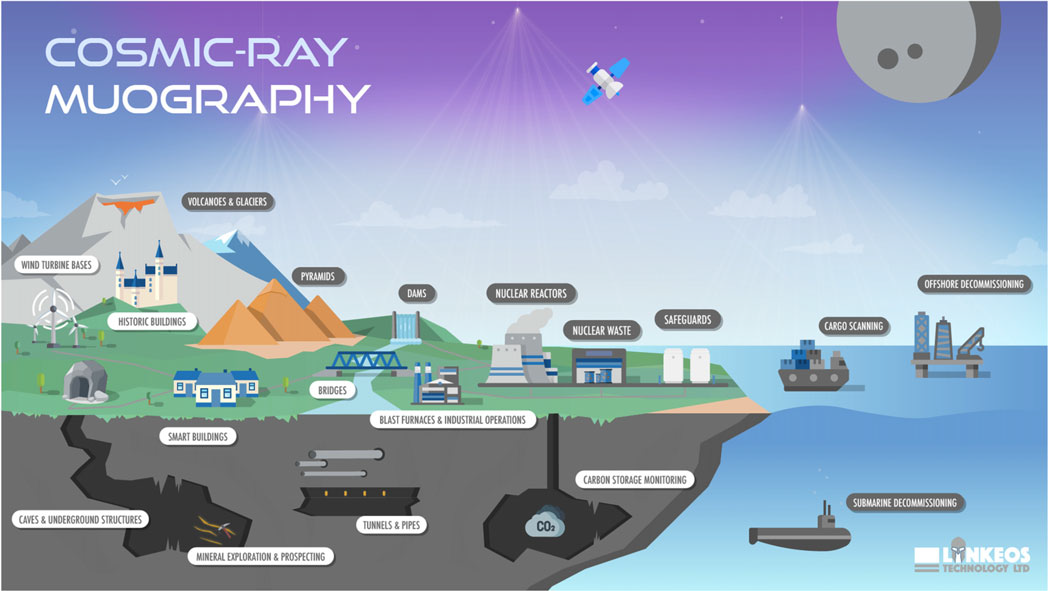
\includegraphics[width=\textwidth]{images/applications.png}
    \caption{Aplicaciones de la muografía. Imagen tomada de (R Kaiser, 2019) \cite{kaiser2019muography}.}
    \label{fig:applications}
\end{figure}

La vulcanología está estrechamente emparentada con el estudio de la corteza terrestre. La corteza es una delgada capa rocosa que cubre la superficie de la Tierra, siendo la capa más externa de la \textbf{geósfera} o tierra sólida. Se separa en dos tipos principales: oceánica y continental. La oceánica tiene un grosor promedio de 6 km, densidad promedio de 3 g cm$^{-3}$ y una edad de menos de 200 millones de años, mientras que la continental tiene un grosor promedio de 39 km, densidad promedio de 2,84 g cm$^{-3}$ y edad promedio de 1500 millones de años \cite{mooney20101}. La corteza terrestre \textit{flota} sobre el manto, teniendo este una densidad mayor. Puesto que la corteza oceánica tiene mayor densidad que la corteza continental, esta última \textit{flota más alto}, y los cuerpos masivos de agua se acumulan sobre la corteza oceánica. Esta condición de equilibrio entre corteza y manto se denomina isostasia. Los elementos más abundantes en la corteza son el oxígeno, el silicio y el aluminio, y los minerales más abundantes son los feldespatos, el cuarzo y los piroxenos \cite{anderson2010geomorphology}.

Como parte de este trabajo, estudiaremos la interacción de las partículas de las EAS con la materia de la corteza terrestre, la cual modelaremos como la denominada \textit{roca estándar}. Esta es una representación genérica del suelo bastante usada en la física de partículas y rayos cósmicos, y el estudio de escaneo de terrenos mediante muones. Se define que la roca estándar está constituida por un material de densidad 2,65 g cm$^{-3}$ aproximadamente, y que cumple las relaciones $\langle Z/A \rangle=0.5$ y $\langle Z^2/A \rangle=5.5$, donde $Z$ y $A$ son el número atómico y el número másico del elemento constituyente respectivamente \cite{groom2001muon}.

En particular, estamos interesados en el fenómeno de \textit{forward scattering} de muones que puede alterar la señal en los detectores; es decir, los muones que se deflectan al interactuar con la materia de la roca. Los muones que son dispersados por \textit{forward scattering} y llegan al detector entorpecen el proceso de escaneo de estructuras geológicas ya que generan señales falsas que no provienen del fondo de muones, como se muestra en la figura \ref{fig:scatteredNoise}. En general, este ruido es significativo para energías por debajo de los 5 GeV, y en simulaciones realizadas por (H Gómez y col. 2018) \cite{gomez2017forward}, observando su efecto de dispersión en una \textit{superficie horizontal}, se vio que aquellos muones con direcciones incidentes cercanas a la tangente del suelo son principalmente los que crean una señal de ruido importante en el detector. Es entonces importante caracterizar este ruido con el fin de reducir su efecto sobre las imágenes de densidades que se deseen tomar de estructuras geológicas. En específico, es necesario analizar el espectro energético y el flujo de los muones que crean este ruido sobre el detector. Para esto, se hará uso de múltiples herramientas computacionales para simular y observar estos efectos. Las herramientas que se utilizarán en el proyecto para las simulaciones son CORSIKA, MAGNETOCOSMICS y Geant4.


%---------------------------------------

\subsection*{Sobre CORSIKA, MAGNETOCOSMICS y Geant4}

CORSIKA\footnote{\textit{\textbf{CO}smic \textbf{R}ay \textbf{SI}mulations for \textbf{KA}scade}} es un programa computacional utilizado para simular EAS causadas por rayos cósmicos. El software utiliza métodos de Montecarlo para simular las interacciones de partículas energéticas de rayos cósmicos con la atmósfera terrestre. Las partículas son rastreadas a lo largo de la atmósfera mientras son sujetas a interacciones con los núcleos de aire y procesos de decaimiento.

El programa hace uso de múltiples modelos diferentes para simular las interacciones, tales como VENUS, QGSJET, DPMJET y SIBYLL para interacciones hadrónicas a altas energías, GHEISHA, FLUKA y UrQMD para interacciones hadrónicas a bajas energías y una adaptación de EGS4 para interacciones electromagnéticas \cite{heck1998corsika}.

Este programa es de uso extendido en el estudio de rayos cósmicos, ya que permite una descripción detallada de las cascadas atmosféricas creadas por estos. La figura \ref{fig:ironcascade} muestra un ejemplo de una cascada producida por la interacción de un núcleo de hierro con la atmósfera, simulada en CORSIKA.

\begin{figure}
    \centering
    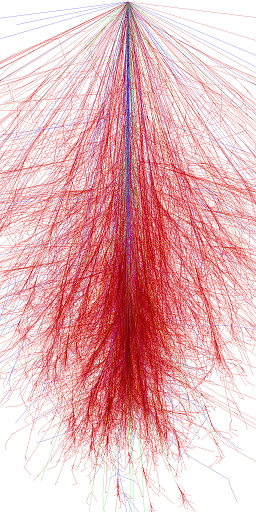
\includegraphics[width=1.5in]{images/ironcascade.png}
    \caption{Cascada atmosférica creada a partir de núcleo de hierro con energía de 1 TeV simulada en CORSIKA. Imagen tomada de \url{https://www.ikp.kit.edu/corsika/index.php}}
    \label{fig:ironcascade}
\end{figure}

Para la simulación de EAS, un aspecto importante es el modelo de rigidez atmosférica. El programa hace seguimiento, entre otras cosas, a la energía de las partículas de las EAS; si una partícula no tiene una energía lo suficientemente alta como para pasar el umbral establecido por el modelo de rigidez atmosférica, la partícula no podrá continuar su viaje a través de la atmósfera. Además, es bien sabido que el campo magnético terrestre puede afectar el viaje de los rayos cósmicos, alterando su curso y desviándolos de sus trayectorias iniciales. Estos son fenómenos cuyos efectos se pueden tener en cuenta en la simulación de EAS mediante la herramienta MAGNETOCOSMICS de Geant4.

La aplicación de MAGNETOCOSMICS permite calcular la trayectoria de partículas cargadas en la magnetosfera terrestre mediante modelos avanzados del campo geomagnético, y computar los modelos de rigidez atmosférica para el filtrado de partículas \cite{magnetocosmics}. La gran utilidad de esta herramienta hace imprescindible integrarla con las simulaciones de CORSIKA.

Finalmente, Geant4\footnote{\textit{\textbf{GE}ometry \textbf{AN}d \textbf{T}racking}} es un grupo de herramientas computacionales (\textit{toolkit}) diseñadas para la simulación del paso de partículas a través de materia, simulando procesos de interacciones y decaimientos. Ha sido ampliamente utilizado en las áreas de física de partículas, física nuclear, física de aceleradores, física espacial y estudios médicos \cite{agostinelli2003geant4}.

En este trabajo balancearemos el uso de todas estas herramientas computacionales para cumplir con los objetivos propuestos en la siguiente sección.









%---------------------------
%\section*{Plan de trabajo}





\section*{Objetivos}

\subsection*{General}
\begin{itemize}
    \item Estimar la contribución del \textit{forward scattering} de muones en la señal registrada por el detector MuTe.
\end{itemize}

\subsection*{Específicos}
\begin{enumerate}
    \item Estimar el flujo de fondo de partículas secundarias a nivel del suelo en el Cerro Machín teniendo en cuenta el efecto del campo geomagnético.
    \item Estimar la señal producida en MuTe debido al flujo de fondo en el Cerro Machín.
    \item Modelar computacionalmente un volumen de materia compuesto de roca estándar y estimar cuánta radiación es producida por el fenómeno de \textit{forward scattering} de muones usando como fuente los muones obtenidos en el objetivo 1.
    \item Calcular si la señal producida por el \textit{forward scattering} de muones en MuTe es estadísticamente significativa respecto de la estimada en el objetivo 2.
\end{enumerate}

\section*{Metodología}

Para un adecuado desarrollo de las actividades propuestas a continuación, es necesario tener un conocimiento de las bases teóricas a aplicar en el proyecto, y de las herramientas que se utilizarán. Por esto, en conjunto con las actividades aquí propuestas, se leerá constantemente y aprenderá sobre la teoría física pertinente para el desarrollo del proyecto; principalmente la teoría concerniente a rayos cósmicos, cascadas atmosféricas extensas, \textit{forward scattering} de muones, detección de rayos cósmicos y el modelo de \textit{roca estándar} a utilizar. De igual manera, se entenderá y analizará el funcionamiento de los \textit{softwares} necesarios, con el fin de tener un buen manejo de estos para llevar a cabo el proyecto. Los programas en cuestión son CORSIKA y MAGNETOCOSMICS para la simulación de EAS, Geant4 para la simulación de interacciones de partículas de las EAS con la materia del suelo, y los códigos desarrollados por la colaboración MuTe para modelar el respectivo detector.

A continuación se presentan las actividades que se proponen para lograr los objetivos expuestos anteriormente.
\subsection*{Actividades}
\begin{enumerate}
    \item Para estimar el flujo de fondo de partículas secundarias en el Cerro Machín se desarrollará un algoritmo computacional que integre los softwares de CORSIKA y MAGNETOCOSMICS permitiendo automatizar y simplificar el proceso de simulación de EAS.
    \item La estimación de la señal que el flujo de fondo de la actividad 1 produce en MuTe se realizará mediante los códigos desarrollados por la colaboración MuTe para modelar el respectivo detector.
    \item El cálculo de la radiación producida por \textit{forward scattering} se realizará a través de las herramientas de simulación de Geant4, para lo cual se elaborará un modelo computacional de roca estándar y se simulará la interacción entre este y los muones de fondo estimados en la actividad 1.
    \item Para determinar si la señal producida por \textit{forward scattering} de muones en el detector MuTe es significativa, se comparará con la señal de fondo estimada en la actividad 2.
    \item La divulgación de los resultados obtenidos se realizará a través del libro de tesis con la teoría, desarrollo y frutos del proyecto pertinentes.
\end{enumerate}

\subsection*{Cronograma de actividades}
\begin{center}
    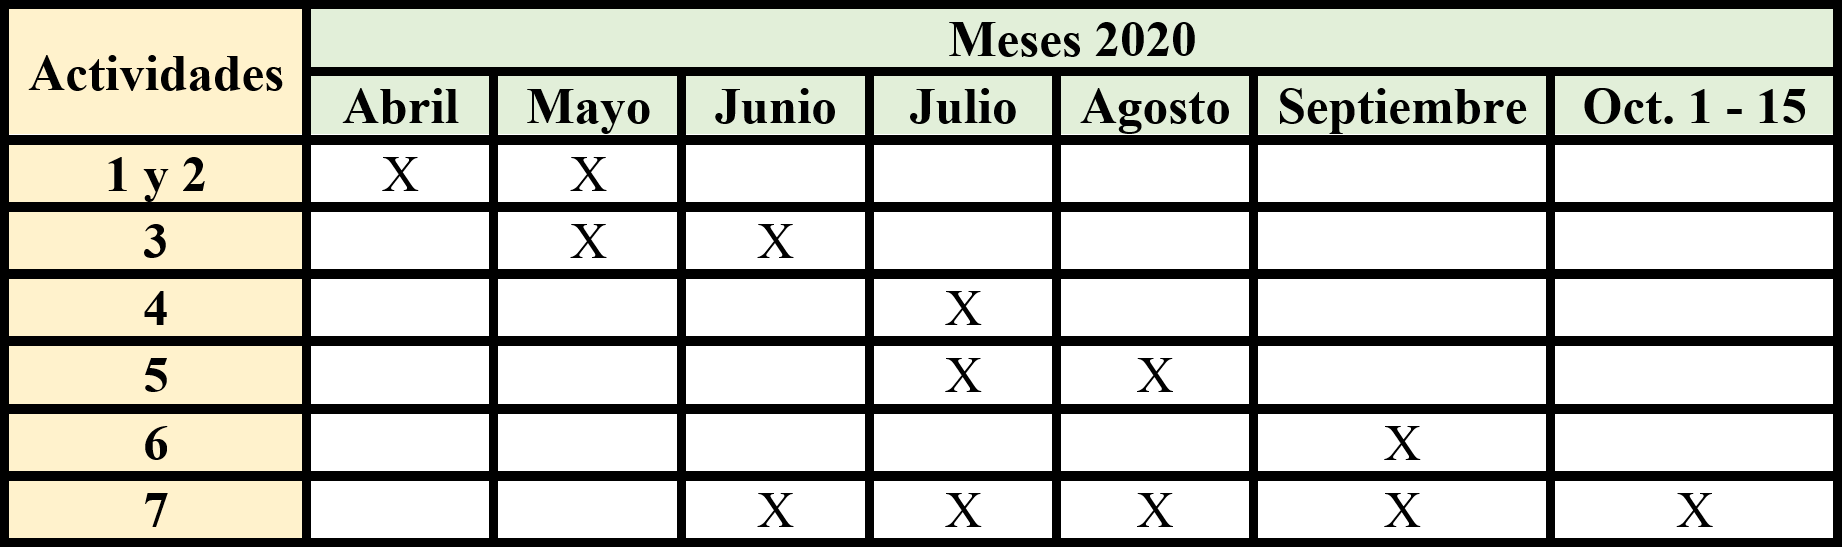
\includegraphics[width=\textwidth]{images/cronograma.png}
\end{center}


\subsection*{Presupuesto}

\begin{center}
    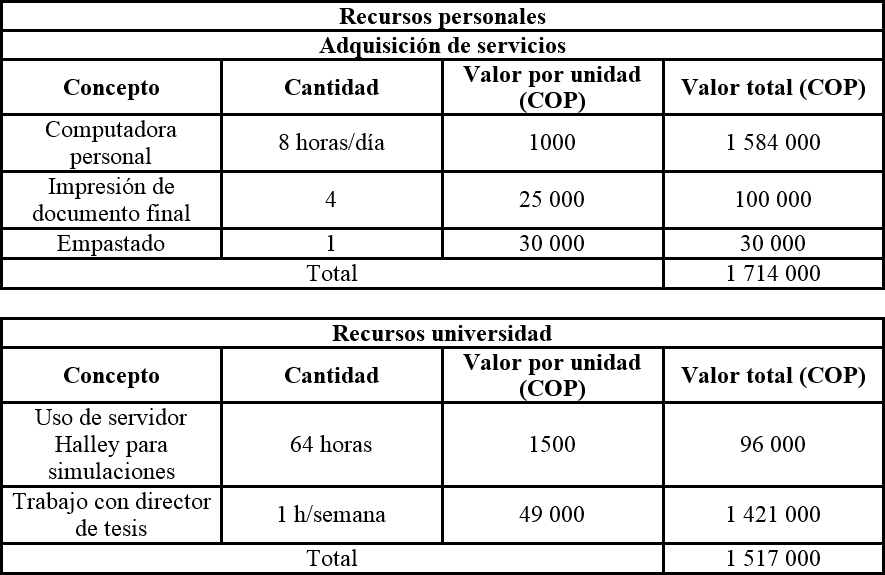
\includegraphics[width=\textwidth]{images/presupuesto.png}
\end{center}



%----------------------------
\printbibliography

\end{document}
